\documentclass[12pt]{article}

\usepackage[english]{babel}
\usepackage[utf8x]{inputenc}
\usepackage{pdfpages}
\usepackage{lastpage} % Required to determine the last page for the footer
\usepackage{extramarks} % Required for headers and footers
\usepackage{graphicx} % Required to insert images
\usepackage{listings} % Required for insertion of code
\usepackage{courier} % Required for the courier font
\usepackage{placeins} % Required to specify float barriers
\usepackage{caption} % Required for table captions

% Margins
\topmargin=-0.45in
\evensidemargin=0in
\oddsidemargin=0in
\textwidth=6.5in
\textheight=9.0in
\headsep=0.25in

\linespread{1.1} % Line spacing

\newcommand{\Title}{Design Documentation} % Assignment title
\newcommand{\Class}{Cos\ 301} % Course/class

\begin{document}

	\vspace{4em}
	
	\begin{center}%
	
	  \LARGE \bf \Title \\[4em]
	  \LARGE {\bf Group 1}\\[1em]
	  \LARGE {\bf Group Members:}\\[2em]
	  \large
	
	     Mbulungo Musetsho				(10176382) \\[1em]
	     Ndivhuwo Ntambeleni			(10001183) \\[1em]
	     Pule Legodi                    (29302732) \\[1em]
	     Lutfiyya Razak				(10198408) \\[1em]
	    	%Enter your details below just as the one above
	
	\end{center}%
	

	\newpage
	\tableofcontents
	
	\newpage
	\section{Background}
		Lecturers assign tutors or teaching assistants, also known as markers, 
		to mark practical’s and assignments. Markers are given a marking sheet 
		with all the students registered for a marking session, which they 
		record the students mark on. The mark sheet is then given to the lecturer
		for publication. However, most of the time the mark sheet is lost or marks
		are not recorded properly. Also there are privacy issues when mark sheets
		are published with all student names, student numbers and marks on it. 
		Because of these issues the client, Jan Kroeze, proposed a mark 
		management system which is accessible from a web browser and mobile devices.
	
		\vspace{0.2in}
	
				 %We must give an introduction of this document
		
		
	
	\section{Vision}
	The purpose of the project is to develop a software solution which provides
a web and mobile platform for markers, students and lecturers handle marks
and marking in the Department of Computer Sciences. It will uphold the
privacy of students so that students cannot see another students mark. It will
reduce paper work and the chances that marks can be lost and provide a
centralized repository for student marks. It will provide functionality to
generate customizable reports at different levels of granularity.
		\vspace{0.2in}
		
			 		 %We must briefly describe the purpose of this document
				
	
	\section{Software Architecture Design}
			%This section needs to demonstrate how the system will be able, within designed software architecture, to address the non-functional requirements.
		\vspace{0.2in}
		
		\subsection{Choices of Technologies}
		%Please refer to the guideline document for some of the items that must be included in this part.
			\vspace{0.2in}
		
		
		\subsection{Chosen Frameworks}
				%Please refer to the guideline document for some of the items that must be included in this part.
				
							 Software architecture framework provides the specification to developers how to organize and display the chosen libraries and design framework of a program. The framework provides a tool for the developers to use during the design of the software to include and implement the non-functional requirements as specified by the master specifications.
							\\
							\\ Object/Relational Mappers
							\begin{itemize}
								 \item Object and relational mappers can be used by the developers to allow the integration and access of repositories without the continuous repetition of code. The mappers serve as a developer defined interface translator, that allows the integration of varies systems without violating the non-functional requirements of security. This technique can be implemented in the design of the program allowing the cross communication from the repositories to the object orientated design.
								
								\item The use of new database with fields from the LDAP repository and CS MySQL database, as specified in the requirement documentation, will be used repetitively in all process interactions (4.1.2). Continues use of these repository lookups can be minimised with the use of ORM model. The integration technique allow the developer to minimise the coding used in the interaction points by separating the query lookup and the implementation of the lookup request. In the implementation of the mappers, the developer must ensure that the data crossover is in the correct format and type as multiple data structures can be accessed that differ from the original data input.
							\end{itemize}
							 Web Frameworks
							\begin{itemize}
								\item Web application framework allows the design and support of dynamic website and web services. As specified by the client, Django web framework will be used for the development of the web services. Django is an open source high level framework that implements the model-view-controller architecture pattern. The application is a Python based program that emphasizes the reusability of code and integration without the need of repetition. The framework implements an Object-relational mapper with a dynamic API for database access.
								
							\end{itemize}
							 Web service frameworks
							\begin{itemize}
							\item Web service framework allows the developer to decentralise inoperability and design front end services for web based applications. Frameworks allow the developer to improve on stability and design and allows connectivity on a word wide basis.
							\item As per client request the web service framework must be an Apache based web service to be allowed to be run on an Apache web server. Apache CXF web service is an open source web service framework that allows the development of services using up frontend programming APIs. The web service allows the incorporation of a variety of protocols such as the SOAP, RESTful HTTP. This conforms to the constraints set by the client in regards to the protocols that must be used in the development of the program.
							
							\end{itemize}
					\vspace{0.2in}	
			
		
		\subsection{Chosen Protocols}
				%Please refer to the guideline document for some of the items that must be included in this part.
			\begin{enumerate}
	                    \item Simple Object Access Protocol (SOAP) \\*
	                    All systems (devices) should be able to access the system’s content through the SOAP-based web services.
	                        \begin{enumerate}
	                            \item The devices (systems) will send a request, procedure call, or a message such as getMark to search or retrieve information (average mark for the module, number of distinctions) through the SOAP-based web services.
	                            \item The SOAP-based web service will process the request or message and send a response to the devices (systems) in a form of a structured XML-based data.
	                        \end{enumerate}
	                    \item Lightweight Directory Access Protocol (LDAP)
	                        \begin{enumerate}
	                            \item It is used to authenticate the system users (Lecturers, Students, and Teaching Assistants) on login for single Sign On.
	                            \item It is used to retrieve the student’s personal details and class lists, including courses assigned to lectures and students.
	                            \item It is used to retrieve system users roles such as, is the user a Lecturer, Student, or teaching assistant for the Module
	                        \end{enumerate}
	                    \item  Hypertext Transfer Protocol over Secure Socket Layer (HTTPS and HTTP)
	                        \begin{enumerate}
	                            \item Used to send and retrieve sensitive data(marks and modules) through a secured (HTTPS) channel.
	                            \item Used to send a GET and POST requests to the web server and web services. Such as adding or updating a student mark.
	                        \end{enumerate}
	
              		\end{enumerate}
			\vspace{0.2in}
			
		
		\subsection{Chosen Libraries}
				%Please refer to the guideline document for some of the items that must be included in this part.
                \begin{enumerate}
					\item Python ldap library \\*
					It is used to integrate LDAP to the Mark sheet system.
						\begin{enumerate}
							\item It provides  a connection to the CS LDAP system for authentication using ldap.initialize() and ldap.open() functionalities.
							\item It also provides a mechanism for retrieving information from the directory, using functions such as LDAPObject.result()
							\item It provides also a list of other LDAP request and response methods
						\end{enumerate}
					\item pyPDF library \\*
					It is a Python library for generating PDFs.
						\begin{enumerate}
							\item It is used to generate pdf files or reports using the python programming language.
							\item It provides different functionalities such as PdfFileWriter class which writes and add pages to the pdf and the merging of different pages.
						\end{enumerate}
					\item MySQLdb Library \\*
					It is a python database library that integrates the MySQL database.
						\begin{enumerate}
							\item It provides functions such as MySQLdb.connect()  for establishing a connection to the MySQL database.
							\item It provides also a methods that executes database queries such as INSERT, DELETE, UPDATE, and SELECT.
						\end{enumerate}
					\item The CSV File library \\*
					It is the python based library, for creating CSV files.
						\begin{enumerate}
							\item It provides the functionality to import and export CSV files.
						\end{enumerate}
				\end{enumerate}
			\vspace{0.2in}

			
	\section{Application Design}
				%must address functional requirements as specied in re-quirements specification.
			\vspace{0.2in}
					
		\subsection{Lower Levels of Granularity Specification}
				\begin{itemize}
					\item User Log In
						\begin{itemize}
						\item View: A log in screen is displayed, wherein the user enters their details then submit to log in. The user will receive a log in result based on the validity of their credentials
						\item Controller: The Controller receives the credentials entered by the user and transfers them to the model for validation. The controller will create a response object based on the validity of the credentials.
						\item Model: The model receives the credentials and simply finds a match from LDAP. It sends the result of the validation back to the controller.
						\end{itemize}
						
					\item Leaf Assessments
					\begin{itemize}
						\item View: On the displayed screen, the user selects one of the following:
						\begin{enumerate}
							\item Add New Leaf Assessment: The user enters all the required information to create a leaf assessment then submits. This will cause a new Assessment to be created and saved into the database, unless there was an error or exception (in which case an exception is thrown and the user is informed of the error)
							\item Search Existing Leaf Assessment (for Update/Delete): If record(s) matching the search were found, they are displayed for the user to update or delete, else then the user is informed of anything that possibly went wrong.
						\end{enumerate}
						\item Controller: The controller receives, based on the kind of operation the user selects, the required information and sends it to the Model for either insertion, update, or deletion.
						\item Model: The model will respectively receive the required information and either save a new leaf assessment, update or delete an existing leaf assessment. After the respective opration, the model will notify the view of changes made to the database.
						
					\end{itemize}
					\item Aggregate Assessment:
						\begin{itemize}
							\item View:The user enters all Aggregate Assessment information as required. When they submit, a new Aggregate Assessment is create based on the specified information.
							\item Controller: The controller uses the provided aggregator to proccess the actual aggregate assessment then it sends it to the Model for storage.
							\item Model: The model receives the aggregate assessment information and provides the controller with the specified aggregator. Then the model receives the processed aggregate assessment and stores it into the database then notifies the user about the results of the operation.
						\end{itemize}
					\item Assessment Reports
						\begin{itemize}
							\item View:The user specifies all required information (including the Freequency Analysis Information) and then submit. They will then choose whether they want it rendered on their device application or downloaded in either PDF or CSV format. Based on their choice of view, the results will be displayed.
							\item Controller: The controller retrieves the report specification submitted by the user and sends it to the model to find matches. The controller will then create a response object with the results and send it to the user for viewing.
							\item Model: The model receives the report specification from the controller and then searches against the database for possible matches then it returns the matches back to the controller.
						\end{itemize}
					\item Student Marks Reports
						\begin{itemize}
							\item View:The user specifies all required information (including aggregation specifications) and then submit. They will then choose whether they want the results rendered on their device application or downloaded in either PDF or CSV format. Based on their choice of view, the results will be displayed.
							\item Controller: The controller retrieves the marks report specification submitted by the user and sends it to the model to find matches. The controller will then create a response object with the results and send it to the user for viewing.
							\item Model: The model receives the marks report specification from the controller and then searches against the database for possible matches then it returns the matches back to the controller.
						\end{itemize}
					\item Audit Reports
						\begin{itemize}
							\item View: The user enters all the specifications for the Audit Report then submit. They will then choose whether they want the results rendered on their device application or downloaded in either PDF or CSV format. Based on their choice of view, the results will be displayed.
							\item Controller: The controller retrieves the Audit Report specifications submitted by the user then send it to the Model to retrieve matches. These matches will be sent back to the controller and then sent back to the user for viewing.
							\item Model: The model receives the Audit Report specifications, retrieves matches of these specifications, and then return them to the controller.
						\end{itemize}
				\end{itemize}
		\vspace{0.2in}
		
		\subsection{API Specifications}
						%UML interfaces and class diagrams for inputs and outputs, etc
						\begin{itemize}
				\item Different API's are to be used throughout the whole project, these are summarised below according to the interface they fall under:
					\begin{itemize}
                                                \item View: Android API, HTTP/HTML 5 API, CSS API.
						\item Controller: Python Django API (Main API). (PHP API and JAVA API might be used under certain conditions).
						\item Model: mySQL API, LDAP API.
					\end{itemize}
			
		\end{itemize}
				\vspace{0.2in}
				
		\subsection{System Class Diagrams }%Ndivhuwo Nthambeleni
		%Class Diagram for assessment marking and assessment aggregation
				
				\begin{itemize}
                                        \item Leaf Assessment, Mark allocation and assessment aggregation Class diagram
                                                \begin{itemize}
                                                \item The class diagram uses the abstact factory design pattern to represent the lower level relationship between an assessment, it's aggregation and the mark allocation.
                                                \item Although all these processes are done in different APIs, this class diagram represents them in a manner that seems like they are on one interface just to make it better to understand.
                                                \end{itemize}
                                        \begin{figure}[h]
                                                \centering
                                                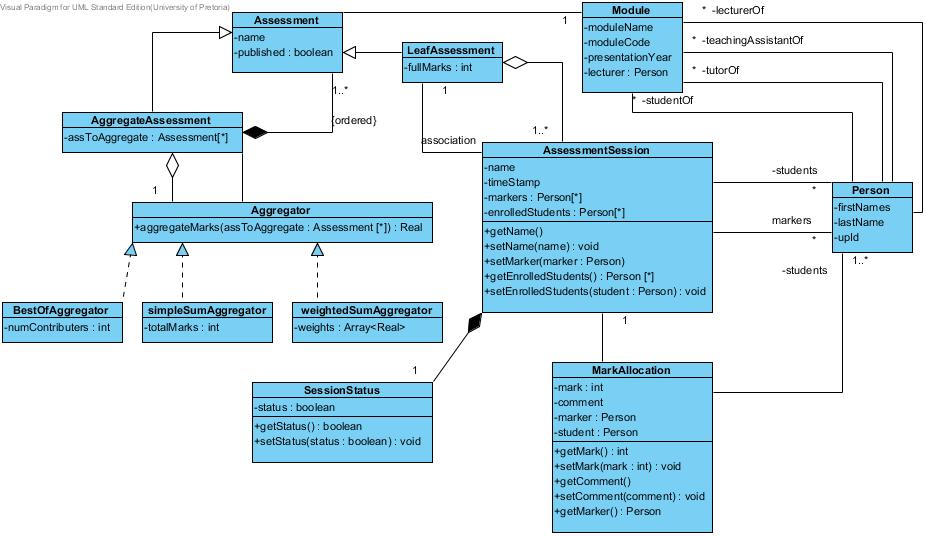
\includegraphics[width=6in, height=4in]{Pictures/MiniPhase2ClassDiag.jpg}
                                                \caption{Assessment Marking and aggregation Class Diagram}
					\end{figure}
					\FloatBarrier
                                        \item Assessment Report Class Diagram
						\begin{itemize}
                                                \item Just like the previous class diagram, this the assessment report class diagram uses the abstract factory design pattern to show how each report is related to a specific assessment.

						\end{itemize}
					\begin{figure}[h]
                                                \centering
                                                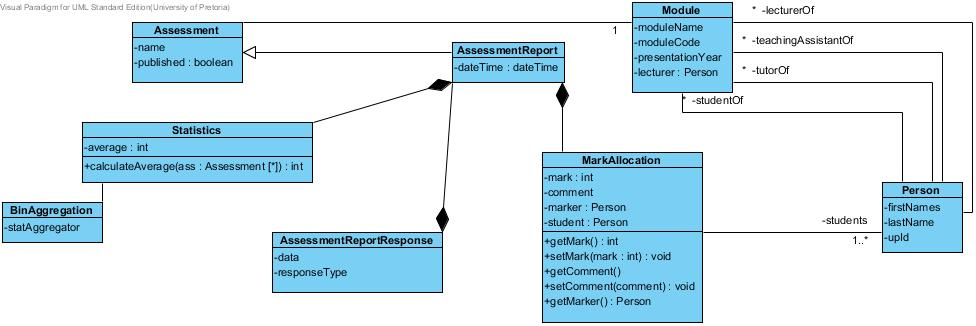
\includegraphics[width=6in, height=4in]{Pictures/assessmentReportClassDiag.jpg}
                                                \caption{Assessment Report Class Diagram}
					\end{figure}
					\FloatBarrier
                                        \item Student Mark Report Class Diagram:
                                                \begin{itemize}
                                                        \item This is an abstract factory class diagram, like the others
							\item Shows how the marks are generated for each student when they are logged on to the system.
						\end{itemize}
					\begin{figure}[h]
                                                \centering
                                                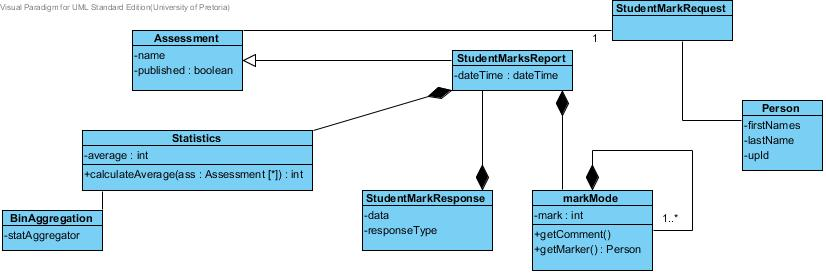
\includegraphics[width=6in, height=4in]{Pictures/studentMarkRequestDiag.jpg}
                                                \caption{Student Mark Report Class Diagram}
					\end{figure}
                     \FloatBarrier
                                \end{itemize}
						%These class diagrams must include attributes, methods and relationships
						
				\vspace{0.2in}
		
		\subsection{System Process Specification}%Mbulungo Muusetsho
						%Sequence and activity diagrams for detailed system process specifications
						\begin{figure}[h]
										\centering
										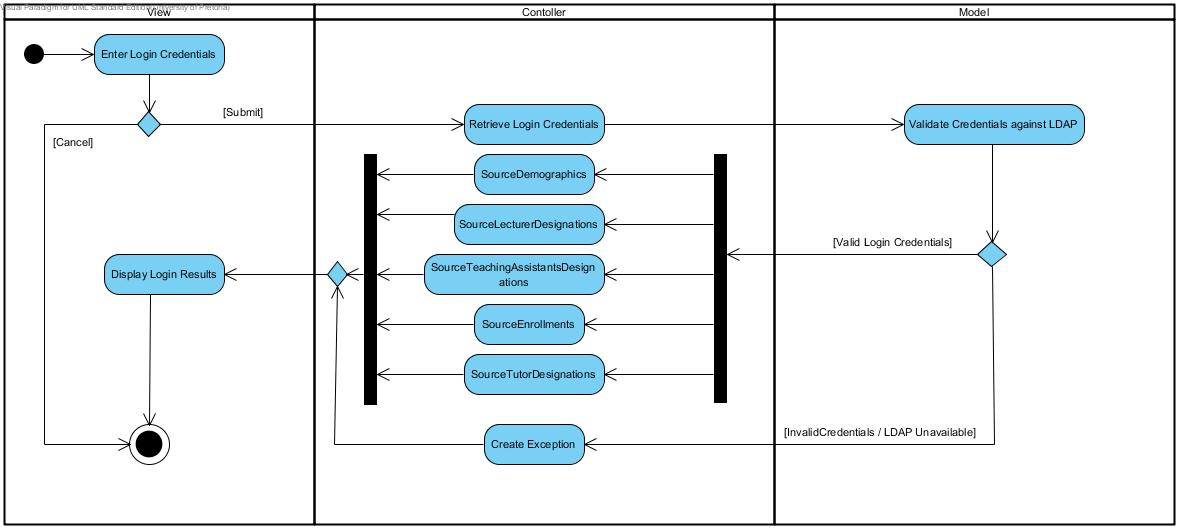
\includegraphics[width=6in, height=4in]{Pictures/LoginActivityDiagram.jpg}
										\caption{User Log In Activity Diagram}
						\end{figure}
						\FloatBarrier
						\begin{figure}[h]
										\centering
										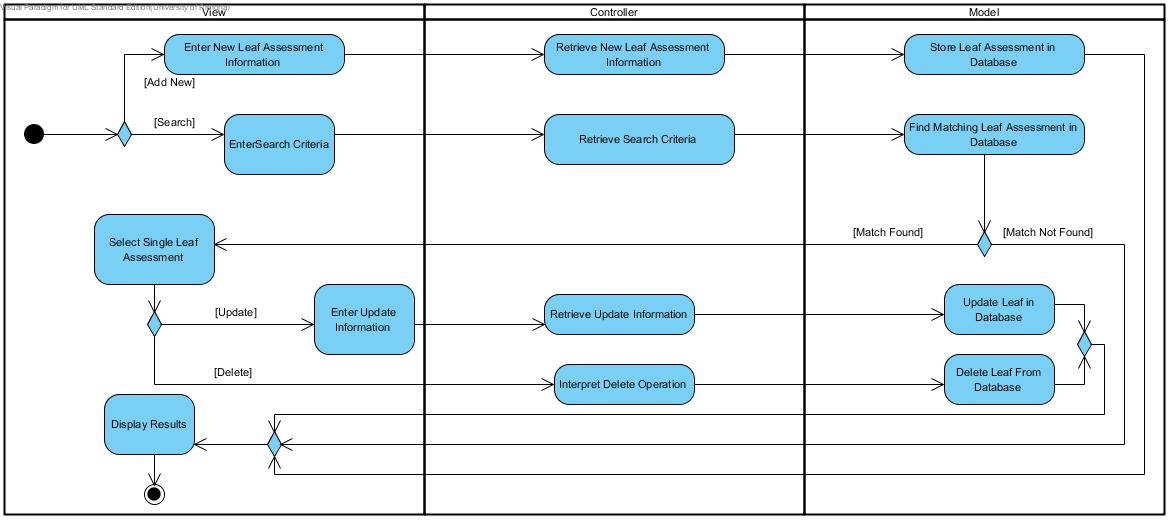
\includegraphics[width=6in, height=4in]{Pictures/LeafAssesmentActivityDiagram.jpg}
										\caption{Leaf Assessment Activity Diagram}
						\end{figure}
						\FloatBarrier
						\begin{figure}[h]
										\centering
										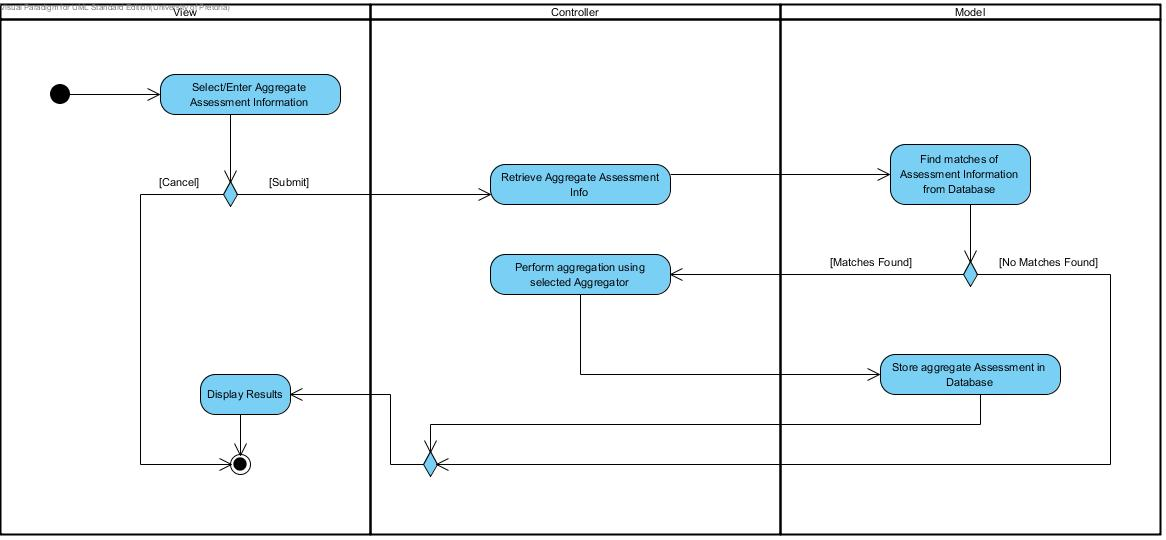
\includegraphics[width=6in, height=4in]{Pictures/AggregateAssesmentActivityDiagram.jpg}
										\caption{Aggregate Assessment Activity Diagram}
						\end{figure}
						\FloatBarrier
						\begin{figure}[h]
										\centering
										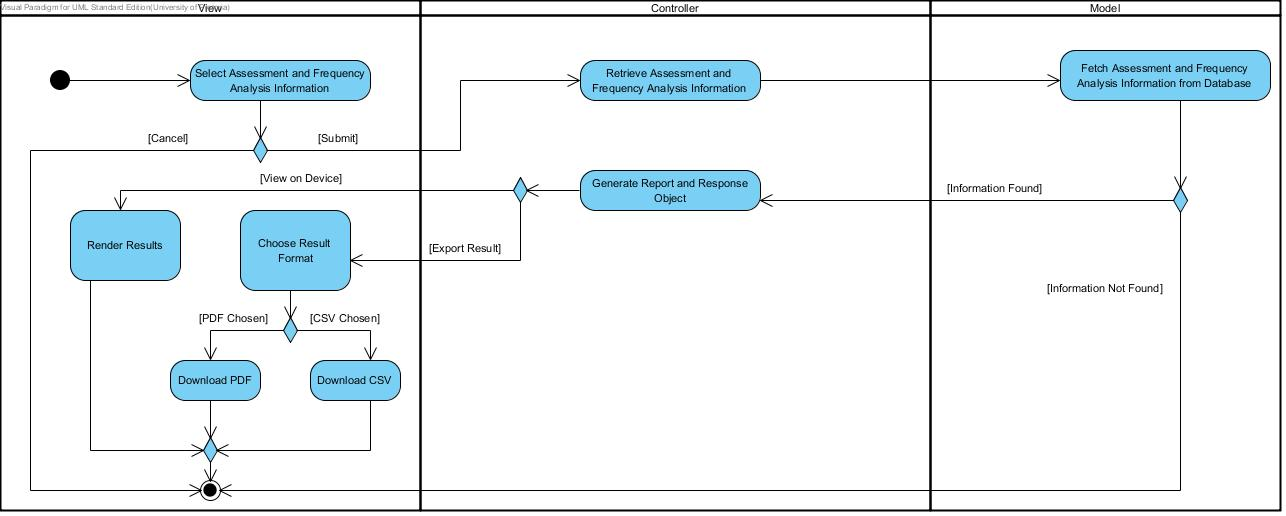
\includegraphics[width=6in, height=4in]{Pictures/AssessmentReportActivityDiagram.jpg}
										\caption{Assessment Report Activity Diagram}
						\end{figure}
						\FloatBarrier
						\begin{figure}[h]
										\centering
										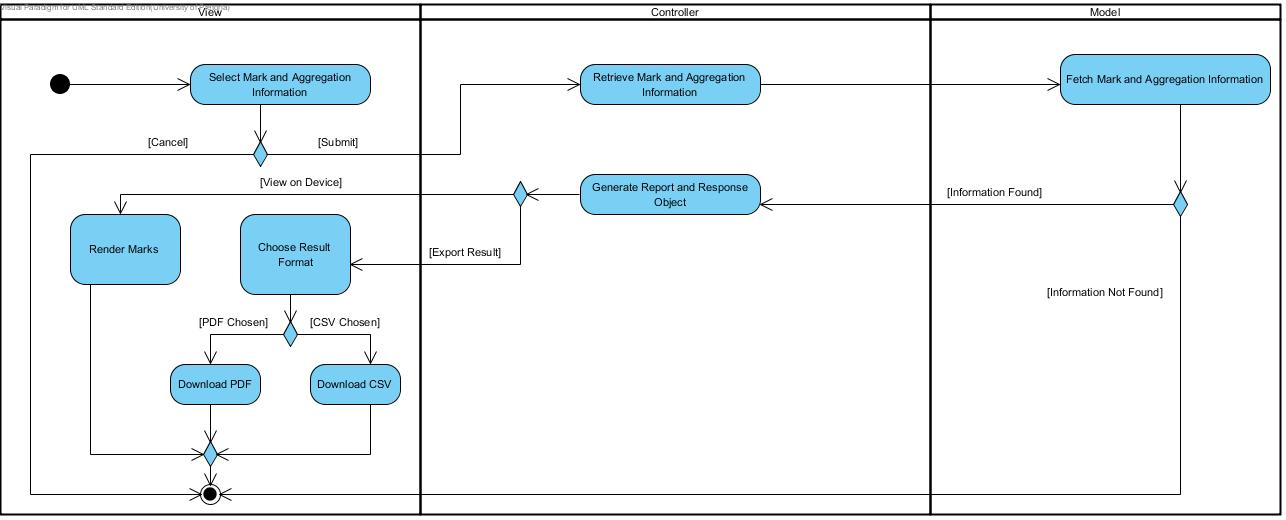
\includegraphics[width=6in, height=4in]{Pictures/StudentMarksReport.jpg}
										\caption{Student Marks Report Activity Diagram}
						\end{figure}
						\FloatBarrier
						\begin{figure}[h]
										\centering
										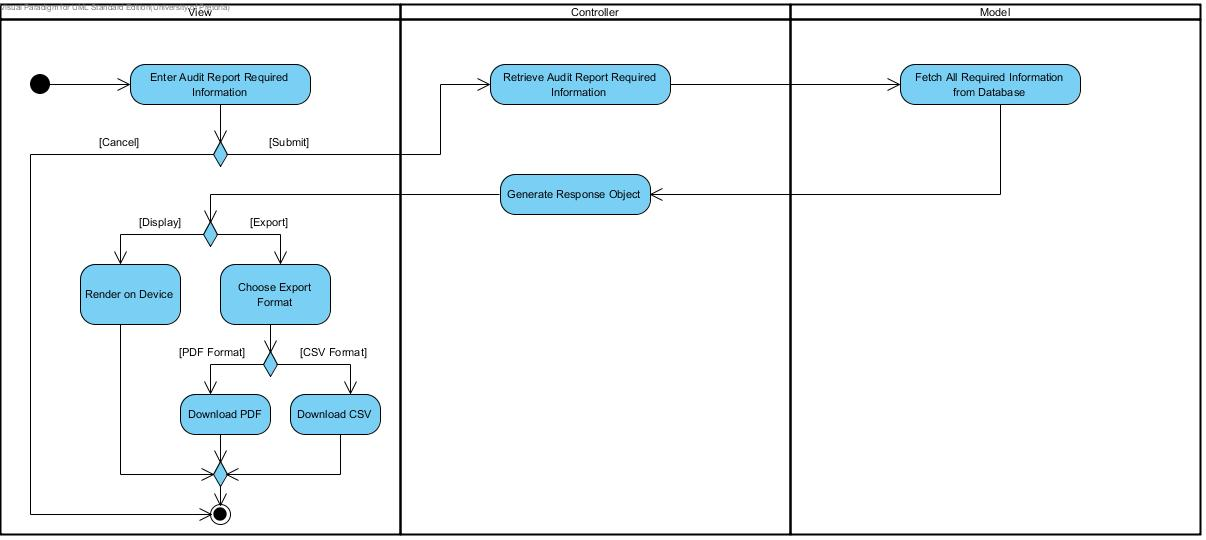
\includegraphics[width=6in, height=4in]{Pictures/AuditReportActivityDiagram.jpg}
										\caption{Audit Report Activity Diagram}
						\end{figure}
				\vspace{0.2in}
		
		\subsection{User Interface Designs} %MatthewHughes and Ndivhuwo Nthambeleni
						%This includes work-flow specifications
						\begin{figure}[h]
										\centering
										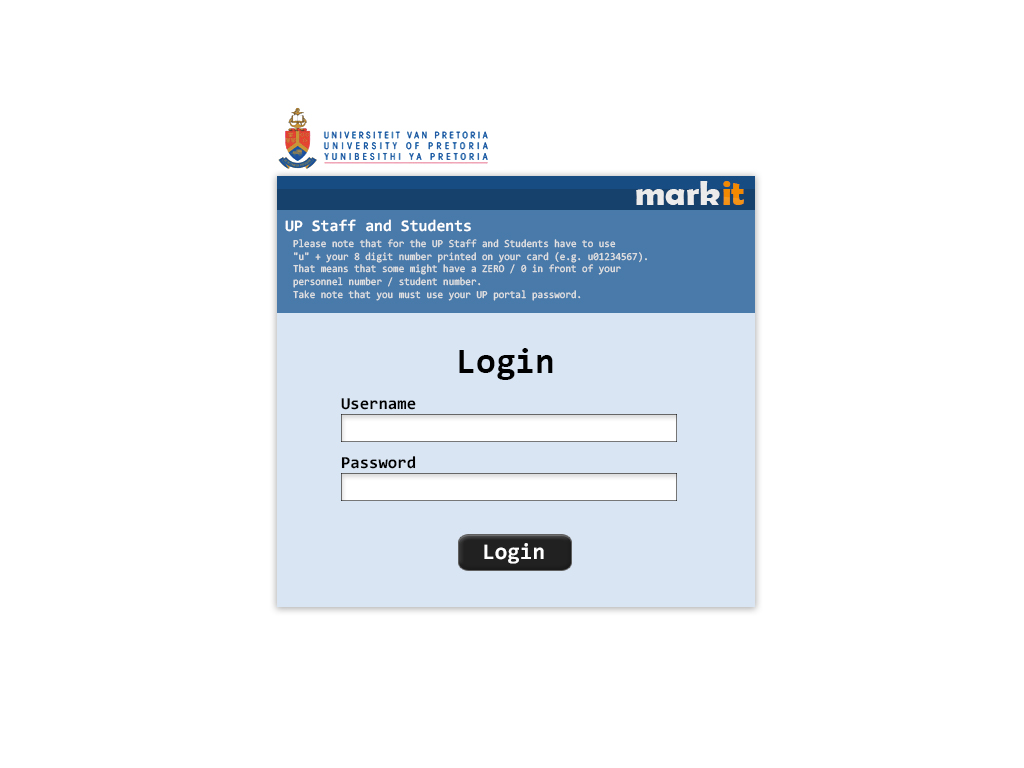
\includegraphics[width=5in, height=3.5in]{Pictures/Screens/Desktop/01logon.jpg}
										\caption{Log In Interface}
						\end{figure}
						\FloatBarrier
						
						\begin{figure}[h]
										\centering
										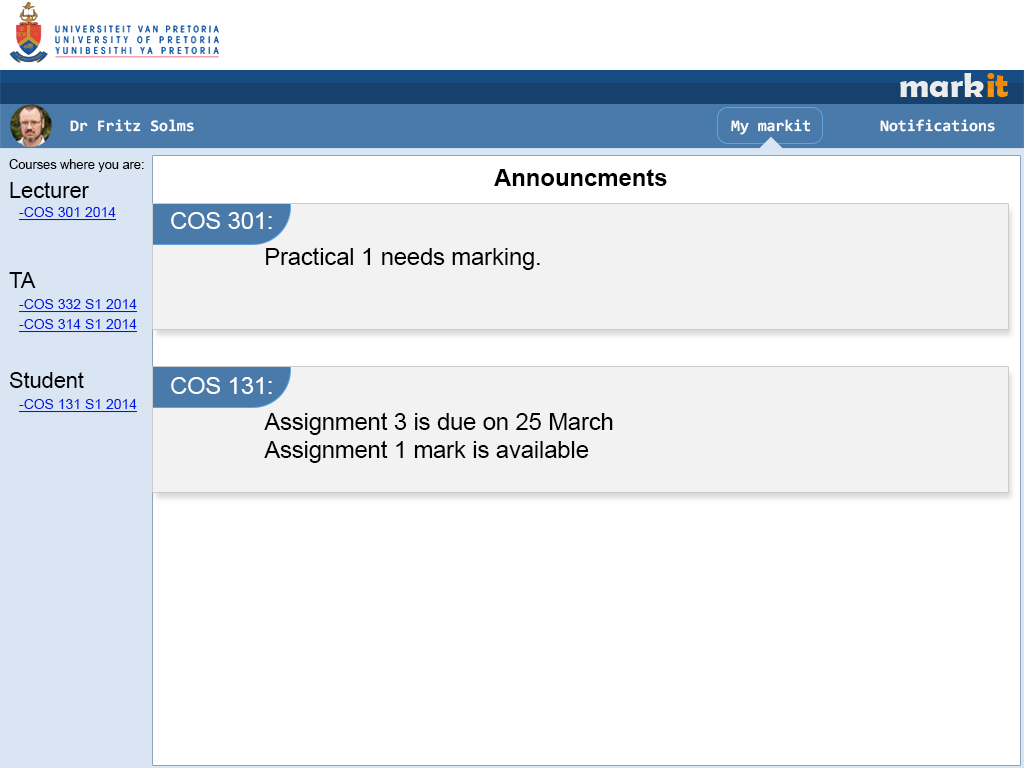
\includegraphics[width=5in, height=3.5in]{Pictures/Screens/Desktop/02homePage.jpg}
										\caption{Home Interface}
						\end{figure}
						\FloatBarrier
						
						\begin{figure}[h]
										\centering
										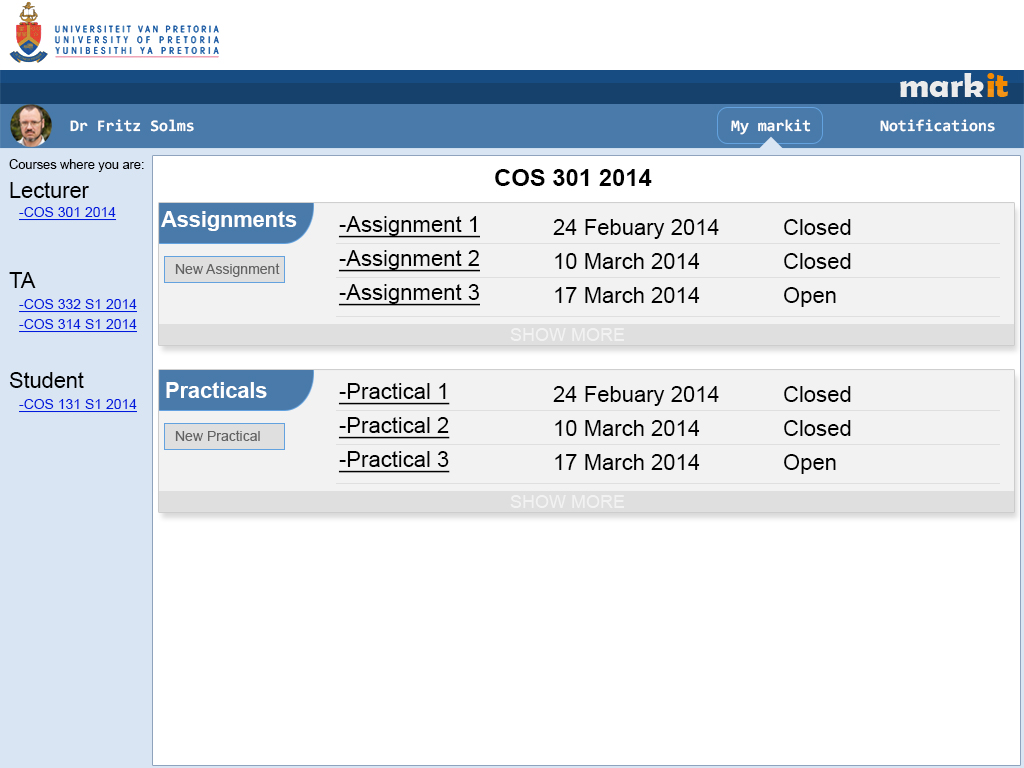
\includegraphics[width=5in, height=3.5in]{Pictures/Screens/Desktop/03subject.jpg}
										\caption{Subject Interface}
						\end{figure}
						\FloatBarrier
						
						\textbf{\begin{figure}[h]
										\centering
										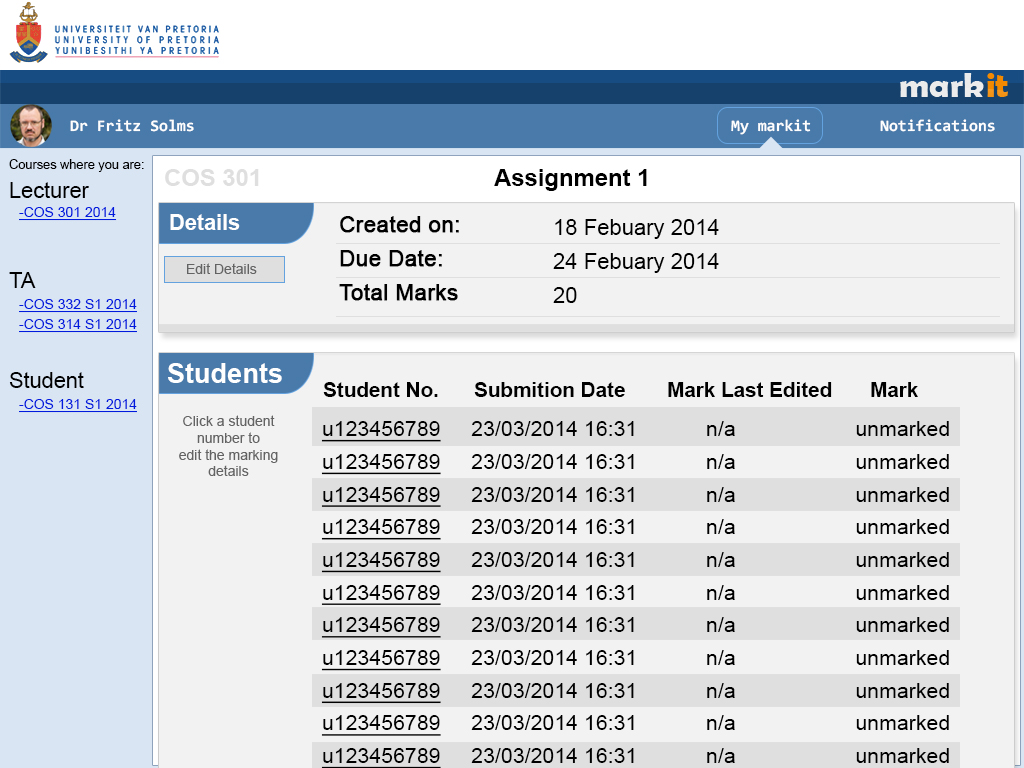
\includegraphics[width=5in, height=3.5in]{Pictures/Screens/Desktop/04assignment.jpg}
										\caption{Assignments Interface}
						\end{figure}
						\FloatBarrier}
						
						\textbf{\begin{figure}[h]
										\centering
										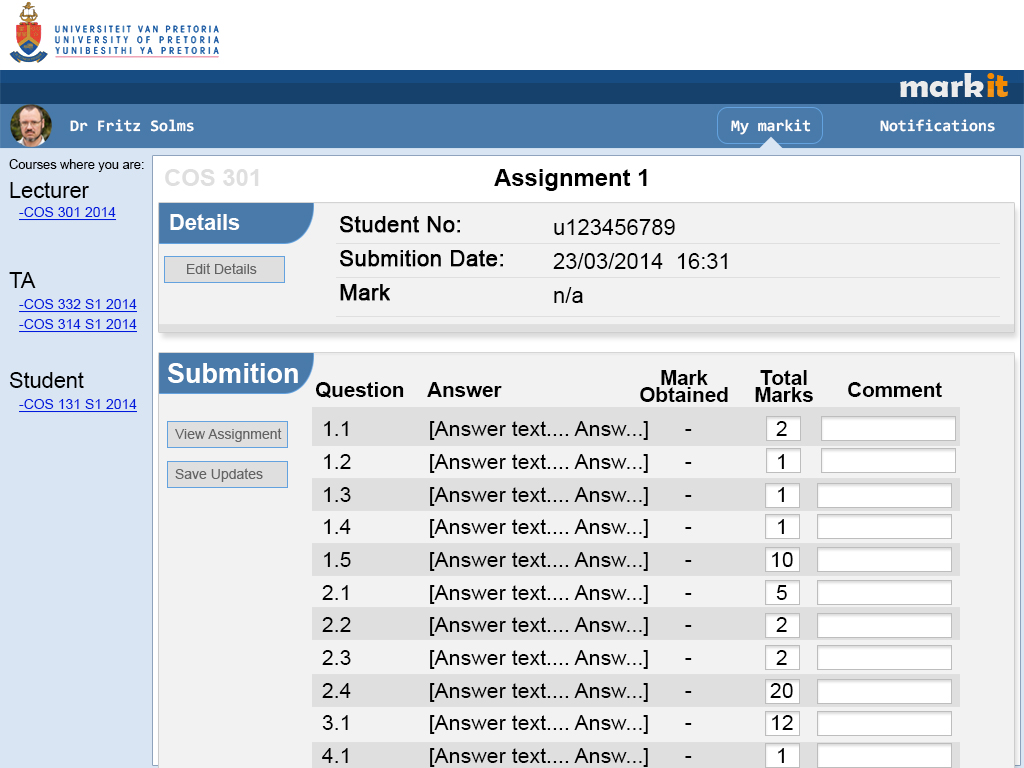
\includegraphics[width=5in, height=3.5in]{Pictures/Screens/Desktop/04assignmentStudent.jpg}
										\caption{Leaf Assignment Interface}
						\end{figure}
						\FloatBarrier}
						
						\textbf{\begin{figure}[h]
										\centering
										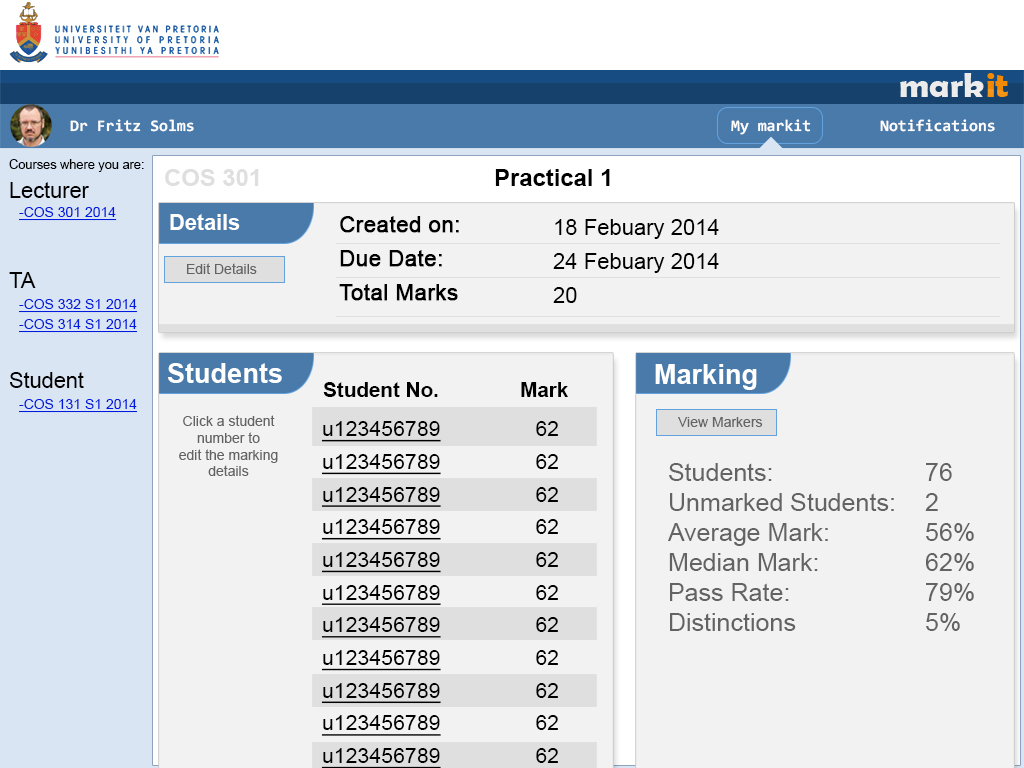
\includegraphics[width=5in, height=3.5in]{Pictures/Screens/Desktop/05practical.jpg}
										\caption{Practicals Interface}
						\end{figure}
						\FloatBarrier}
						
						\textbf{\begin{figure}[h]
										\centering
										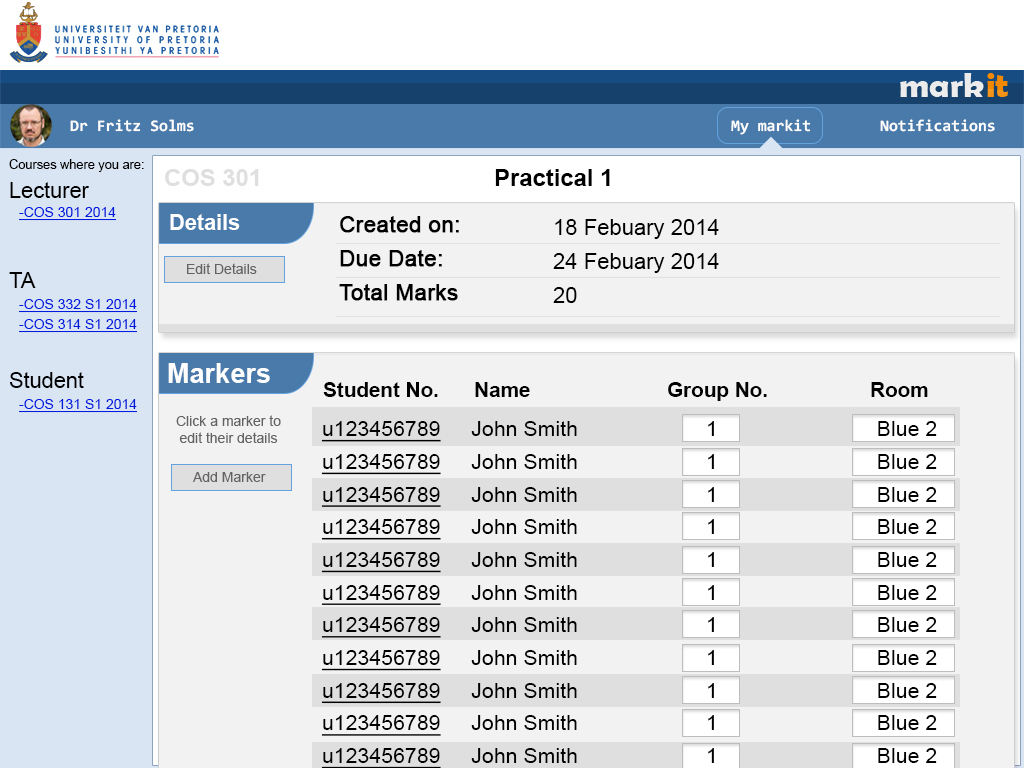
\includegraphics[width=5in, height=3.5in]{Pictures/Screens/Desktop/05practicalMarkers.jpg}
										\caption{Practical Markers Interface}
						\end{figure}
						\FloatBarrier}
				\vspace{0.2in}
		\newpage
		\subsection{Database Desgin} %Lutfiyya
						
				
					\captionof{table}{Module}
					\begin{tabular}{|p{1.0in}|p{0.9in}|p{0.5in}|p{0.4in}|p{1.0in}|p{1.1in}|} \hline
					Field & Type & Null & Key & Default & Extra \\ \hline
					id & int(11) & No & Primary & Null & auto\_increment \\ \hline
					code & varchar(20) & No &  & 0 &  \\ \hline
					name & varchar(20) & No &  & Null &  \\ \hline
					lecturer  & varchar(20) & No &  & 0 &  \\ \hline
					description & text & Yes &  & Null &  \\ \hline
					semester & smallint(6) & No &  & 0 &  \\ \hline
					has\_webct & tinyint(4) & Yes &  & Null &  \\ \hline
					year\_group & int(11) & Yes &  & Null &  \\ \hline
					hidden & tinyint(3) unsigned & No &  & 0 &  \\ \hline
					last\_updated & datetime & No &  & 0000-00-00 00:00:00 &  \\ \hline
					discussion\_board & tinyint(4) & Yes &  & Null &  \\ \hline
					tutors\_allowed & tinyint(2) & Yes &  & Null &  \\
					\hline
					\end{tabular}



					\captionof{table}{Session}
					\begin{tabular}{|p{1.0in}|p{0.9in}|p{0.5in}|p{0.4in}|p{1.0in}|p{1.1in}|} \hline
					Field & Type & Null & Key & Default & Extra \\ \hline
					id & int(11) & No & Primary & Null & auto\_increment \\ \hline
					code & varchar(20) & No &  & 0 &  \\ \hline
					marker & varchar(20) & No &  & Null &  \\ \hline
					status\_open & bool & No &  & 0 &  \\ \hline
					start\_time & datetime & No &  & 0000-00-00 00:00:00 &  \\ \hline
					end\_time & datetime & No &  & 0000-00-00 00:00:00 &  \\ \hline
					assessment\_id & int(11) & No & Foreign & Null &  \\ \hline
					session\_number & int(11) & No &  & Null &  \\ \hline
					\end{tabular}
					
					
					\newpage
					\captionof{table}{Assessment}
					\begin{tabular}{|p{1.0in}|p{0.9in}|p{0.5in}|p{0.4in}|p{1.0in}|p{1.1in}|} \hline
					Field & Type & Null & Key & Default & Extra \\ \hline
					assessment\_id & int(11) & No & Primary & Null & auto\_increment \\ \hline
					type & varchar(11) & No &  & 0 &  \\ \hline
					description & text & Yes &  & Null &  \\ \hline
					assessment\_name & varchar(11) & No &  & 0 &  \\ \hline
					code & varchar(11) & No &  & 0 &  \\ \hline
					date\_issued & datetime & No &  & 0000-00-00 00:00:00 &  \\ \hline
					date\_due & datetime & No &  & 0000-00-00 00:00:00 &  \\ \hline
					mark\_id & int(11) & No & Foreign & Null &  \\ \hline
					submission\_details & text & No &  & Null &  \\ \hline
					\end{tabular}
					
					\captionof{table}{Mark Allocation}
					\begin{tabular}{|p{1.0in}|p{1.0in}|p{0.4in}|p{0.4in}|p{1.0in}|p{1.1in}|} \hline
					Field & Type & Null & Key & Default & Extra \\ \hline
					mark\_id & int(11) & No & Primary & Null & auto\_increment \\ \hline
					mark & varchar(10) & Yes &  & 0 &  \\ \hline
					comment & varchar(30) & Yes &  & 0 &  \\ \hline
					marker\_name & varchar(20) & No &  & 0 &  \\ \hline
					timestamp & datetime & No &  & 0000-00-00 00:00:00 &  \\ \hline
					totalMark & varchar(20) & No &  & 0 &  \\ \hline
					\end{tabular}
					
					
					
					\captionof{table}{Simple Sum Aggregator}
					\begin{tabular}{|p{1.0in}|p{1.0in}|p{0.4in}|p{0.5in}|p{0.9in}|p{1.1in}|} \hline
					Field & Type & Null & Key & Default & Extra \\ \hline
					ssa\_id & int(11) & No & Primary & Null & auto\_increment \\ \hline
					assessment\_id & int(11) & No & Foreign & Null &  \\ \hline
					Num\_of\_questions & varchar(20) & No &  & 0 &  \\ \hline
					full\_marks & varchar(20) & No &  & 0 &  \\ \hline
					\end{tabular}
					
					
					
					\captionof{table}{Weighted Sum Aggregator}
					\begin{tabular}{|p{1.0in}|p{0.9in}|p{0.4in}|p{0.6in}|p{0.9in}|p{1.1in}|} \hline
					Field & Type & Null & Key & Default & Extra \\ \hline
					wsa\_id & int(11) & No & Primary & Null & auto\_increment \\ \hline
					assessment\_id & int(11) & No & Foreign & Null &  \\ \hline
					num\_of\_assessements & varchar(20) & No &  & 0 &  \\ \hline
					calculate\_weights & int(11) & No &  & Null &  \\ \hline
					\end{tabular}
					
					
					\newpage
					\captionof{table}{Best Of Aggregator}
					\begin{tabular}{|p{1.0in}|p{1.0in}|p{0.4in}|p{0.5in}|p{0.9in}|p{1.1in}|} \hline
					Field & Type & Null & Key & Default & Extra \\ \hline
					boa\_id & int(11) & No & Primary & Null & auto\_increment \\ \hline
					assessement\_id & int(11) & No & Foreign & Null &  \\ \hline
					Best\_aggregates & varchar(20) & No &  & 0 &  \\ \hline
					sum\_marks & varchar(20) & No &  & 0 &  \\ \hline
					\end{tabular}
					
					
					
					
					\captionof{table}{Student Report}
					\begin{tabular}{|p{1.0in}|p{1.0in}|p{0.4in}|p{0.4in}|p{1.0in}|p{1.1in}|} \hline
					Field & Type & Null & Key & Default & Extra \\ \hline
					sReport\_id & int(11) & No & Primary & Null & auto\_increment \\ \hline
					timestamp & datetime & No &  & 0000-00-00 00:00:00 &  \\ \hline
					assessment\_name & varchar(11) & No & Foreign & 0 &  \\ \hline
					ssa\_id & int(11) & No & Foreign & Null &  \\ \hline
					wsa\_id & int(11) & No & Foreign & Null &  \\ \hline
					\end{tabular}
					
					
					
					\captionof{table}{Audit Report}
					\begin{tabular}{|p{1.1in}|p{0.9in}|p{0.5in}|p{0.4in}|p{1.0in}|p{1.1in}|} \hline
					Field & Type & Null & Key & Default & Extra \\ \hline
					ar\_id & int(11) & No & Primary & Null & auto\_increment \\ \hline
					datestamp & datetime & No &  & 0000-00-00 00:00:00 &  \\ \hline
					userId & int(11) & No &  & Null &  \\ \hline
					action\_performed & varchar(30) & Yes &  & 0 &  \\ \hline
					assessment\_CRUD & varchar(30) & No &  & 0 &  \\ \hline
					sessions\_CRUD & varchar(30) & No &  & 0 &  \\ \hline
					mark\_CRUD & varchar(30) & No &  & 0 &  \\ \hline
					session\_status\_request & varchar(30) & yes &  & 0 &  \\ \hline
					publish\_mark\_request & varchar(30) & Yes &  & 0 &  \\ \hline
					report\_request & varchar(30) & Yes &  & 0 &  \\ \hline
					\end{tabular}
					
					
					\captionof{table}{Assessement Report}
					\begin{tabular}{|p{1.0in}|p{1.0in}|p{0.4in}|p{0.4in}|p{1.0in}|p{1.1in}|} \hline
					Field & Type & Null & Key & Default & Extra \\ \hline
					as\_id & int(11) & No & Primary & Null & auto\_increment \\ \hline
					datestamp & datetime & No &  & 0000-00-00 00:00:00 &  \\ \hline
					class\_average & varchar(20) & No &  & 0 &  \\ \hline
					frequency\_analysis & varchar(20) & No &  & 0 &  \\ \hline
					assessement\_id & int(11) & No & Foreign & Null &  \\ \hline
					\end{tabular}
				\vspace{0.2in}
			
			
	
	
		
		
	\newpage
	\section{Glossary}
		\begin{tabular}{|p{2.1in}|p{2.2in}|} \hline 
			Term & Defintion \\ \hline 
			Android & A smart phone operating system developed by Google. It is used by a variety of mobile phone manufacturers including HTC, Sony, etc. \newline  \\ \hline 
			API & Application Programming Interface \\ \hline 
			CS & Computer Science \\ \hline 
			CSS & Cascading Style Sheet \\ \hline 
			Database & A collection of all information that is necessary to the functioning of a system \\ \hline 
			granularity & Extent to which a system is broken down into small parts \\ \hline 
			HTML & HyperText Markup Language \\ \hline 
			HTTP & Hypertext Transfer Protocol \\ \hline 
			LDAP & Lightweight Directory Access Protocol \newline  \\ \hline 
			MySQL & ~open-source~relational database management system~(RDBMS) \\ \hline 
			ORM & Object-Relational Mapping \\ \hline 
			repository & central place where data is stored and maintained \\ \hline 
			RESTful & Representational state transfer \\ \hline 
			SOAP & Simple Object Access Protocol \newline  \\ \hline 
			XML & Extensible Markup Language \\ \hline 
		\end{tabular}

		\vspace{0.2in}
		
			
	
	
\end{document}
